\chapter{\label{cha:sts_siamese_neural_networks}Siamese Neural Networks for STS}

\section{Introduction}
A \textit{Siamese Neural Network} is a class of neural network architectures that contain two or more identical subnetworks which is usually employed in applications that requires comparisons between two or more inputs (signature verification, image similarity etc.). The network can take two or more inputs at the same time and they will be processed by different subnetworks at the same time. The subnetworks have the same configuration with the same parameters and weights. The training process is mirrored across all the subnetworks which means that the parameters remain same with all the subnetworks. Each subnetwork contains a traditional perceptron model like LSTM, CNN etc. The neural network compares the output of the two subnetworks through a distance metric like a cosine distance and the error is back-propagated. In the testing phase, the neural network predicts whether the two inputs are different through this similarity measure. 

Siamese neural networks have been employed in many applications in different areas like signal processing \cite{thiolliere2015hybrid, 8461524, 8268960, 8453811, 10.1007/978-3-319-66429-3_11, 8064706, 8268994, Zeghidour2016}, biology \cite{10.1093/bioinformatics/bty887, Szubert2019}, chemistry and pharmacology \cite{10.1093/bioinformatics/btz411}, geometry \cite{10.1093/jcde/qwaa003}, computer vision  \cite{6797067,1467314,rs10020355,21be1428c6a44fb7a32d49ba83126bcb,6976727,6636646,Taigman_2014_CVPR,7163112,8269987,HANIF201954}, physics \cite{Zou18, DEBAETS2019645}, robotics \cite{Utkin2017, 7970671, 8461044}, video processing \cite{AAAI1816790, 8036238, Liu2018, 8587153} etc. They have also been used in NLP tasks \cite{10.5555/2018936.2018965,10.1145/3209978.3210144,Gonzalez2019} including STS \cite{das-etal-2016-together, neculoiu-etal-2016-learning, Mueller_Thyagarajan_2016}. In fact, the best result in the SICK dataset \cite{marelli-etal-2014-semeval} was provided by a Siamese neural network \cite{Mueller_Thyagarajan_2016} which shows that state-of-the-art in STS is Siamese neural networks. 

In addition to providing state-of-the-art results in STS, there are additional advantage in using Siamese neural networks. As we mentioned before, in Siamese neural networks, as the weights are shared across subnetworks there are fewer parameters to train, which in turn means they require less training data and less tendency to over-fit. Given the amount of human labour required to produce datasets for STS, Siamese neural networks can provide the ideal solution for the STS task. As the second advantage, the Siamese neural network architecture when trained on a STS task, can be adopted as sentence encoders. The output vector of the subnetwork is a semantically rich vector representation of the input sentence \cite{Mueller_Thyagarajan_2016}. These advantages motivates us to explore Siamese neural network architectures more in STS. 


We address four research questions in this chapter:

\textbf{RQ1:} Can existing state-of-the-art Siamese neural network architecture be modified to provide better STS results?

\textbf{RQ2:} Can the method further improved with transfer learning and data augmentation techniques?

\textbf{RQ3:} Can the proposed Siamese neural network be easily adopted in to different languages?

\textbf{RQ4:} How well the proposed Siamese neural network perform in a different domain? 


The main contributions of this chapter are as follows.

\begin{enumerate}
	\item We propose a GRU (Gated recurrent unit) based Siamese neural network that outperforms state-of-the-art LSTM based Siamese neural network in small STS datasets. 
	
	\item We propose a LSTM (Long short-term memory) and Self-attention based Siamese neural network that outperforms state-of-the-art LSTM based Siamese neural network in large STS datasets.
	
	\item We propose further enhancements to the architecture using transfer learning and data augmentation.  
	
	\item We evaluate how well the proposed Siamese neural network architecture performs in different languages and domains. 
	
	\item The initial findings of this chapter is published in \citet{ranasinghe-etal-2019-semantic}. 
	
	\item The code and the pre-trained models are publicly available to the community\footnote{The public GitHub repository is available on \url{https://github.com/tharindudr/Siamese-recurrent-rrchitectures}}
\end{enumerate}


The rest of this chapter is organised as follows. Section \ref{sec:siamese_related} describes the past research done with Siamese neural networks. Section \ref{sec:siamese_method} discusses the methodology and the experiments done with three English STS datasets. Section \ref{sec:siamese_transfer} and \ref{sec:siamese_aug} provides more experiments to improve the results. Experiments done with other languages and domains are shown in Section \ref{sec:siamese_languages} and Section \ref{sec:siamese_domains}. The chapter finishes with conclusions and ideas for future research directions in Siamese neural networks. 


\section{Related Work}
\label{sec:siamese_related}

The Siamese neural networks have been very popular in the machine learning community. The first appearance of Siamese neural networks date back to 1994. It was first introduced by \citet{doi:10.1142/S0218001493000339} to detect forged signatures. By comparing two handwritten signatures, this Siamese neural network was able to predict if the two signatures were both original or if one was a forgery. Even before that, \citet{6797067} introduced a similar artificial neural network able to recognize fingerprints, though by a different name. 

Siamese neural networks have been applied in various applications after that. In audio and speech signal processing field, \citet{thiolliere2015hybrid} merged a dynamic-time warping based spoken term discovery (STD) system with a Siamese deep neural network for automatic discovery of linguistic units from raw speech, \citet{8461524} used a Siamese model to detect all the semantically similar audio clips in an input audio recording and \citet{8268960} employed a Siamese model to recognize Arabic dialects from Arabic speech content found in media broadcasts. In biology, \citet{10.1093/bioinformatics/bty887} implemented a Siamese neural network to compare DNA sequences and recently \citet{Szubert2019} present a Siamese neural network-based technique for visualization and interpretation of single-cell datasets. Image analysis is the field with the highest number of applications for the Siamese neural networks. Recognising fingerprints \cite{6797067}, similar image detection \cite{1467314,rs10020355,21be1428c6a44fb7a32d49ba83126bcb,6976727,6636646}, face verification \cite{Taigman_2014_CVPR}, gesture recognition \cite{7163112}, hand writing analysis \cite{8269987} and patch matching \cite{HANIF201954} are some of them. As you can observe, all of these tasks involve in comparing two or more things.

Recently, Siamese neural networks have been employed in NLP too. \citet{10.5555/2018936.2018965} proposed similarity Learning via Siamese Neural Network (S2Net), a technique able to discriminatingly learn concept vector representations of text words. \citet{10.1145/3209978.3210144} used Siamese neural network to recognize clickbaits in online media outlets. \citet{Gonzalez2019} proposed a natural language processing application of the Siamese neural network for extractive summarization, which means that their technique can extrapolate most relevant sentences in a document. Not limited to those applications Siamese neural networks have been implemented in STS tasks too in NLP. \citet{das-etal-2016-together} used a CNN based Siamese neural network to detect similar questions on question and answer websites such as Yahoo Answers, Baidu, Zhidao, Quora, and Stack Overflow. \citet{neculoiu-etal-2016-learning} employed a Siamese neural network based on Bidirectional LSTMs to identify similar job titles. The baseline we used for this chapter; MALSTM \cite{Mueller_Thyagarajan_2016} uses a LSTM based Siamese neural network to perform semantic textual similarity and it provides the best results for SICK dataset outperforming other STS methods like Tree-LSTMs \cite{tai-etal-2015-improved}. They use the exponent of the negative Manhattan distance between two outputs from the two subnetworks as the similarity function. Due to the performance this can be considered as the state-of-the-art Siamese neural network for STS. However, this architecture leaves considerable room for variation which we exploit in this chapter as we explain in Section \ref{sec:siamese_method}.



\section{Exploring Siamese Neural Networks for STS}
\label{sec:siamese_method}

The basic structure of the Siamese neural network architecture used in our experiments is shown in Figure \ref{fig:siamese}. It consists of an embedding layer which represents each sentence as a sequence of word vectors. This sequence of word vectors is then fed into a Recurrent Neural Network (RNN) cell which learns a mapping from the space of variable length sequences of 300-dimensional vectors into a 50 dimensional vector. The sole error signal back propagated during training, stems from the similarity between these 50 dimensional vectors, which can be also used as a sentence representation. Initially, the similarity function we used was based on Manhattan distance. To make sure that the prediction is between 0 and 1, we took the exponent of the negative Manhattan distance between 2 sentence representations. The similarity function was adopted from \citet{Mueller_Thyagarajan_2016}. The proposed variants of our architecture are:


\begin{enumerate}
	\item LSTM - Block A in Figure \ref{fig:siamese} contains a single LSTM cell. This is the architecture suggested by \citet{Mueller_Thyagarajan_2016} 
	
	\item Bi-directional LSTM - Block A in Figure \ref{fig:siamese} contains a single Bi-directional LSTM cell. Bi-directional LSTM tends to understand the context better than Unidirectional LSTM \cite{650093}.
	
	\item GRU - Block A in Figure \ref{fig:siamese} contains a single GRU cell. GRUs have been shown to exhibit better performance on smaller datasets \cite{Chung2014EmpiricalEO}. 
	
	\item Bi-directional GRU - Block A in Figure \ref{fig:siamese} contains a single Bi-directional GRU cell. Bi-directional GRUs tend to understand the context better than Unidirectional GRU ~\cite{vukotic:hal-01351733}.
	
	\item LSTM + Attention - Block A in Figure \ref{fig:siamese} contains a single LSTM cell with self attention \cite{NIPS2017_3f5ee243}.
	
	\item GRU + Attention - Block A in Figure \ref{fig:siamese} contains a single GRU cell with self attention \cite{NIPS2017_3f5ee243}.
	
	\item GRU + Capsule + Flatten - Block A in Figure \ref{fig:siamese} contains a GRU followed by a capsule layer and a flatten layer. Dynamic routing used between capsules performs better than a traditional max-pooling layer \cite{NIPS2017_2cad8fa4}.
	
\end{enumerate}

\begin{figure}[ht]
	\centering
	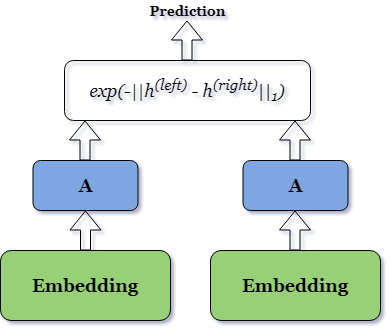
\includegraphics[scale=0.5]{figures/semantic_textual_similarity/siamese_neural_networks/siamese_architecture.png}
	\caption[Basic structure of the Siamese neural network]{Basic structure of the Siamese neural network. Unit A is changed over the architectures.}
	\label{fig:siamese}
\end{figure}
	
	
	As the word embedding model we used Word2vec embeddings \cite{DBLP:journals/corr/abs-1301-3781} pre-trained on Google news corpus\footnote{Pretrained Word2vec can be downloaded from \url{https://code.google.com/archive/p/word2vec/}}. We represented each word as a 300 lengthened vector using this model. For the words that do not appear in this model we used a random vector. We evaluated all the above variations in the three English STS datasets we introduced in \ref{cha:sts_introduction}; SICK, STS 2017 and QUORA. We trained the Siamese models on the training sets on those datasets and evaluated them on the testing sets. The results are shown in Table \ref{tab:sick_siamese}, Table \ref{tab:sts_siamese} and Table \ref{tab:quora_siamese} respectively. 
	
	 
	\begin{table*}[htb]
		%\footnotesize
		\centering
		\scalebox{0.95}{
			\begin{tabular}{|l|cc|}
				\hline
				\textbf{Model} & $\bm{\rho}$   & $\bm{\tau}$     
				\\ \hline
				\textit{LSTM}                  
				& 0.802 & 0.733  \\
				\textit{Bi-LSTM}                     
				& 0.784 & 0.708   \\
				\textit{GRU}                     
				& 0.838$^{\dagger}$ & 0.780$^{\dagger}$  \\
				\textit{Bi-GRU}                     
				& 0.832 & 0.773  \\
				\textit{LSTM + Attention}                     
				& 0.827  & 0.765       \\
				\textit{GRU + Attention}                     
				& 0.818  & 0.751       \\
				\textit{GRU + Capsule + Flatten}                     
				& 0.806  & 0.733       \\
				\hline
			\end{tabular}
		}
		\caption[Results for SICK with Siamese Neural Network]{Results for SICK dataset with different variants of Siamese Neural Network. For each variant, Pearson Correlation ($\bm{\rho}$) and Spearman Correlation ($\bm{\tau}$) are reported between the predicted values and the gold labels of the test set. Best result from all the variations is marked with ${\dagger}$.}  
		\label{tab:sick_siamese}
	\end{table*}
	
	
	\begin{table*}[htb]
		%\footnotesize
		\centering
		\scalebox{0.95}{
			\begin{tabular}{|l|cc|}
				\hline
			\textbf{Model} & $\bm{\rho}$   & $\bm{\tau}$     
			\\ \hline
			\textit{LSTM}                  
			& 0.831 & 0.762  \\
			\textit{Bi-LSTM}                     
			& 0.784 & 0.708   \\
			\textit{GRU}                     
			& 0.853$^{\dagger}$ & 0.811$^{\dagger}$  \\
			\textit{Bi-GRU}                     
			& 0.844 & 0.804  \\
			\textit{LSTM + Attention}                     
			& 0.830  & 0.791       \\
			\textit{GRU + Attention}                     
			& 0.825  & 0.782       \\
			\textit{GRU + Capsule + Flatten}                     
			& 0.806  & 0.765       \\
			\hline
			\end{tabular}
		}
		\caption[Results for STS 2017 with Siamese Neural Network]{Results for STS 2017 dataset with different variants of Siamese Neural Network. For each variant, Pearson Correlation ($\bm{\rho}$) and Spearman Correlation ($\bm{\tau}$) are reported between the predicted values and the gold labels of the test set. Best result from all the variations is marked with ${\dagger}$. }  
		\label{tab:sts_siamese}
	\end{table*}
	
	
	\begin{table*}[htb]
		%\footnotesize
		\centering
		\scalebox{0.95}{
			\begin{tabular}{|l|c|}
				\hline
				\textbf{Model} & RMSE     
			\\ \hline
			\textit{LSTM}                  
			& 0.412   \\
			\textit{Bi-LSTM}                     
			& 0.402    \\
			\textit{GRU}                     
			& 0.415  \\
			\textit{Bi-GRU}                     
			& 0.408   \\
			\textit{LSTM + Attention}                     
			& 0.382$^{\dagger}$        \\
			\textit{GRU + Attention}                     
			& 0.398       \\
			\textit{GRU + Capsule + Flatten}                     
			& 0.421        \\
			\hline
			\end{tabular}
		}
		\caption[Results for QUORA with Siamese Neural Network]{Results for QUORA dataset with different variants of Siamese Neural Network. For each variant, Root Mean Squared Error (RMSE) reported between the predicted values and the gold labels of the test set. Best result from all the variations is marked with ${\dagger}$. }  
		\label{tab:quora_siamese}
	\end{table*}
	
As can be seen in Table \ref{tab:sick_siamese} and \ref{tab:sts_siamese}, for SICK and STS 2017 datasets, GRU based Siamese neural network model outperformed the LSTM based Siamese neural network model which we used as a baseline and this provided the best result. It can be seen that complex architectures that involves Bi-directional RNNs, Attention and Capsule mechanisms did not perform well compared to the simple architectures like GRU. We can conclude that for the smaller datasets like STS 2017 and SICK, GRU based architecture performs better because GRU has less parameters than LSTM \cite{Chung2014EmpiricalEO}. With less parameters, the architecture does not need a lot of training instances to optimise the training process.

However, when it comes to the big STS dataset; QUORA, the way that the variants of the Siamese neural network behaves is different. As we introduced in Chapter \ref{cha:introduction}, QUORA was the biggest STS dataset we experimented which has 320,000 training instances. As a result, even the complex architectures like RNNs with Attention get the opportunity to optimise their parameters and deliver good results. This can be seen in Table \ref{tab:quora_siamese}. For the QUORA dataset, LSTM + Attention based Siamese neural network model outperformed the LSTM based Siamese neural network model which we used as a baseline and this provided the best result. For bigger datasets, we can conclude that Siamese neural networks based on LSTM with Attention would outperform Siamese neural networks only with LSTMs. 

From the experimented variants, one notable observation is the poor performance of capsules in Siamese architectures. Despite providing good results in many NLP tasks like text classification \cite{NIPS2017_2cad8fa4,hettiarachchi-ranasinghe-2019-emoji} capsule based variant fails to outperform the simple LSTM based variant even in the bigger STS dataset. This implies that capsule based Siamese neural networks won' be a good fit for STS tasks.

With these findings we answer our \textbf{RQ1} in this chapter. We have improved the state-of-the-art Siamese neural network architecture and propose a GRU based Siamese neural network architecture for the smaller STS datasets and LSTM+Attention based Siamese neural network for larger STS datasets.

			
\subsection{Impact of Transfer Learning}
\label{sec:siamese_transfer}
Transfer learning is a machine learning method where a model developed for a task is reused as the starting point for a model on a second task. It is a popular approach in deep learning where pre-trained models are used as the starting point for a new task. This is usually done in the scenarios where there is not enough data to train a neural network so that starting from already tuned weights would be advantageous \cite{pmlr-v97-houlsby19a, ruder-etal-2019-transfer}. Transfer learning has often provided good results for smaller datasets. Therefore, we explored the impact of transfer learning, with Siamese neural networks in STS. 

We saved the weights of the models that were trained on each STS dataset; SICK, STS 2017 and QUORA. We specifically used the two models that performed best in these dataset; Siamese neural network with GRU and Siamese neural network with LSTM + Attention. We again initiated training for each dataset, however rather than training from scratch, we used the weights of the models trained on other STS dataset. We compared this transfer learning results to the results we got from training the model from scratch. We conducted this transfer learning experiment only on STS2017 and SICK dataset since the QUORA dataset was already big and transfer learning from a smaller dataset to a larger dataset won't make much sense.


\begin{table*}[htb]
	%\footnotesize
	\centering
	\scalebox{0.95}{
		\begin{tabular}{|l|c|c|}
			\hline
			\textbf{Start Model} & STS2017 & SICK      
			\\ \hline
			\textit{STS2017$_{GRU}$}                  
			& 0.853 & \textcolor{gray}{(+0.01)} \\
			\textit{STS2017$_{LSTM+Aten}$}                     
			& 0.830 & \textcolor{gray}{(+0.01)}  \\
			\hline
			\textit{SICK$_{GRU}$}                     
			& \textcolor{gray}{(+0.01)} & 0.838 \\
			\textit{SICK$_{LSTM+Aten}$}                     
			& \textcolor{gray}{(+0.01)} & 0.827 \\
			\hline
			\textit{QUORA$_{GRU}$}                     
			& \textcolor{gray}{(-0.02)}  &  \textcolor{gray}{(-0.02)}    \\
			\textit{QUORA$_{LSTM+Aten}$}                     
			& \textcolor{gray}{(-0.04)} &  \textcolor{gray}{(-0.04)}    \\
			\hline
		\end{tabular}
	}
	\caption[Results for transfer learning with Siamese Neural Network]{Results for transfer learning with different variants of Siamese Neural Network. For each transfer learning experiment we show the difference between with transfer learning and without transfer learning. Non-grey values are the results of the experiments without transfer learning which we showed in the previous section too. We only report the Pearson correlation due to ease of visualisation.}  
	\label{tab:transfer_siamese}
\end{table*}

As can be seen in Table \ref{tab:transfer_siamese} some of the transfer learning experiments improved the results for STS2017 and SICK datasets with both architectures. When we performed transfer learning from STS2017 $\Rightarrow$ SICK and SICK $\Rightarrow$ STS2017 the results improve. This shows that transfer learning can improve the results in Siamese neural networks. However, when we performed transfer learning from QUORA $\Rightarrow$ STS2017 and QUORA $\Rightarrow$ SICK the results did not improve, in fact, they decrease, despite QUORA being the largest STS dataset we experimented. This finding somewhat controversial to the general belief in the community that transfer learning from a larger dataset improves the result. In this case, we believe that this happens due to the fact that the QUORA dataset is very different to the other two datasets as we discussed in Chapter \ref{cha:sts_introduction}. Despite QUORA having a large number of training instances, when performing transfer learning, the neural network finds it difficult to optimise the weights for STS2017 and SICK that were already optimised for a very different dataset; QUORA. This result in a decrease in the result. On the other hand transfer learning between STS2017 and SICK improved the results for both datasets since they are similar in nature as we discussed in Chapter \ref{cha:sts_introduction}. 

Therefore, we can conclude that transfer learning can improve the results for Siamese neural networks in STS. However, the transfer learning dataset should be picked carefully considering the similarity of the two datasets too, rather than only considering the size of the dataset.


\subsection{Impact of Data Augmentation}
\label{sec:siamese_aug}
As we observed before, the neural networks perform better when there is a large number of training instances. Therefore, many approaches have been taken to increase the number of training instances. Usually this has resulted better performance with neural networks \cite{wei-zou-2019-eda}. Therefore, we experimented the impact of data augmentation with the Siamese neural network architectures we proposed before. We only conducted this experiment with STS 2017 and SICK datasets as QUORA already has a large number of training instances.

We employed thesaurus-based augmentation in which 10,000 additional training examples are generated by replacing random words with one of their synonyms found in Wordnet \cite{10.1145/219717.219748}. A similar approach has been successfully adopted by \citet{Mueller_Thyagarajan_2016, 10.5555/2969239.2969312} too.  We specifically used the two models that performed best with the bigger dataset and smaller dataset; Siamese neural network with GRU and Siamese neural network with LSTM + Attention. Since the transfer learning improved the results in previous experiment, we trained the augmented training set on the transferred models; models trained on STS2017 for SICK experiments and models trained on SICK for STS2017. 


\begin{table*}[htb]
	%\footnotesize
	\centering
	\scalebox{0.95}{
		\begin{tabular}{|c|c|c|}
			\hline
		   \textbf{Dataset} &	\textbf{Start Model} &  $\bm{\rho}$      
			\\ \hline
		\multirow{ 2}{*}{\textit{SICK}}	& \textit{STS2017$_{GRU}$}                  
			& \textcolor{gray}{(+0.01)} \\
		 &	\textit{STS2017$_{LSTM+Aten}$}                     
			& \textcolor{gray}{(+0.01)}  \\
			\hline
			\multirow{ 2}{*}{\textit{STS2017}}  & \textit{SICK$_{GRU}$}                     
			& \textcolor{gray}{(+0.01)}  \\
			& \textit{SICK$_{LSTM+Aten}$}                     
			& \textcolor{gray}{(+0.01)} \\
			\hline
		\end{tabular}
	}
	\caption[Results for data augmentation with Siamese Neural Network]{Results for data augmentation with different variants of Siamese Neural Network. For each data augmentation experiment we show the difference between with dat augmentation and without data augmentation. We only report the Pearson correlation ($\bm{\rho}$) due to ease of visualisation.}  
	\label{tab:augmentation_siamese}
\end{table*}

As can be seen in the results, data augmentation improved the results of all the experiments. However, even with the additional 10,000 training instances, GRU based Siamese neural network outperformed LSTM + Attention based Siamese neural network. We can conclude that simple data augmentation techniques can improves the performance of Siamese neural networks in STS task. From the Siamese neural network experiments we conducted, our best result for both STS2017 and SICK datasets were provided by GRU based Siamese neural network when combined with both transfer learning and data augmentation.

This answers our \textit{RQ2} in this Chapter, we can use transfer learning and simple data augmentation techniques to improve the results of Siamese neural networks in STS. 

\begin{table*}[htb]
	%\footnotesize
	\centering
	\scalebox{0.95}{
		\begin{tabular}{|l|c|}
			\hline
			\textbf{Model} & $\bm{\rho}$      
			\\ \hline
			\citet{jimenez-etal-2014-unal} & 0.807 \\
			\citet{bjerva-etal-2014-meaning} & 0.827 \\
			\citet{zhao-etal-2014-ecnu-one} & 0.841 \\
			\textit{Siamese LSTM} & 0.863  \\
			\textit{Siamese GRU} & 0.882  \\
			\hline
		\end{tabular}
	}
	\caption[Results comparison for SICK with leader board results]{Results for SICK dataset with different variants of Siamese Neural Network. For each variant, Pearson Correlation ($\bm{\rho}$) is reported between the predicted values and the gold labels of the test set.}  
	\label{tab:sick_siamese_all}
\end{table*}

\begin{table*}[htb]
	%\footnotesize
	\centering
	\scalebox{0.95}{
		\begin{tabular}{|l|c|}
			\hline
			\textbf{Model} & $\bm{\rho}$      
			\\ \hline
			\citet{tian-etal-2017-ecnu} & 0.851 \\
			\textit{Siamese LSTM} & 0.852  \\
			\citet{maharjan-etal-2017-dt} & 0.854 \\
			\citet{cer-etal-2017-semeval}  & 0.855   \\
			\textit{Siamese GRU} & 0.862  \\
			\hline
		\end{tabular}
	}
	\caption[Results comparison for STS2017 with leader board results]{Results for STS2017 dataset with different variants of Siamese Neural Network. For each variant, Pearson Correlation ($\bm{\rho}$) is reported between the predicted values and the gold labels of the test set.  }  
	\label{tab:sts_siamese_all}
\end{table*}

Furthermore, we compared the results of the best Siamese neural network variant with the best results submitted to the competitions \cite{cer-etal-2017-semeval, marelli-etal-2014-semeval} and with the unsupervised STS methods we have experimented so far in this part of the thesis. As can be seen in Table \ref{tab:sick_siamese_all} and \ref{tab:sts_siamese_all} GRU based Siamese neural network architecture outperforms the best system submitted to both competition. It also outperforms the unsupervised STS methods we have so far explored in this part of the thesis. Therefore, we can conclude that Siamese architecture is currently the best system we have experimented so far for English STS.


\section{Portability to Other Languages}
\label{sec:siamese_languages}
Our \textit{RQ3} targets the multilinguality aspect of the proposed approach; \textit{Can the proposed Siamese neural network be easily adopted in to different languages?}. To answer this, we evaluated our method in Arabic STS and Spanish STS datasets that were introduced in Chapter \ref{cha:sts_introduction}. Our approach has the advantage that it does not rely on language dependent features.  As a result, the approach is easily portable to other languages given the availability of pre-trained word embedding models in that particular language. As word embedding models we used AraVec \cite{SOLIMAN2017256} \footnote{AraVec has been trained on Arabic Wikipedia articles. The models are available on \url{https://github.com/bakrianoo/aravec}} for Arabic and Spanish 3B words Word2Vec Embeddings \cite{doi:10.1177/1550147718811827}\footnote{Spanish 3B words Word2Vec Embeddings have been trained on Spanish news articles, Wikipedia articles and Spanish Boletín Oficial del Estado (BOE; English: Official State Gazette). The model is available on \url{https://github.com/aitoralmeida/spanish_word2vec}} for Spanish.


\begin{table*}[htb]
	%\footnotesize
	\centering
	\scalebox{0.95}{
		\begin{tabular}{|l|cc|}
			\hline
			\textbf{Model} & $\bm{\rho}$   & $\bm{\tau}$     
			\\ \hline
			\textit{LSTM}                  
			& 0.746 & 0.690  \\
			\textit{Bi-LSTM}                     
			& 0.725 & 0.683   \\
			\textit{GRU}                     
			& 0.763$^{\dagger}$ & 0.723$^{\dagger}$  \\
			\textit{Bi-GRU}                     
			& 0.752 & 0.717  \\
			\textit{LSTM + Attention}                     
			& 0.741  & 0.703       \\
			\textit{GRU + Attention}                     
			& 0.739  & 0.691       \\
			\textit{GRU + Capsule + Flatten}                     
			& 0.712  & 0.679       \\
			\hline
		\end{tabular}
	}
	\caption[Results for Arabic STS with Siamese Neural Network]{Results for Arabic STS dataset with different variants of Siamese Neural Network. For each variant, Pearson Correlation ($\bm{\rho}$) and Spearman Correlation ($\bm{\tau}$) are reported between the predicted values and the gold labels of the test set. Best result from all the variations is marked with ${\dagger}$. }  
	\label{tab:arabic_siamese}
\end{table*}


	\begin{table*}[htb]
	%\footnotesize
	\centering
	\scalebox{0.95}{
		\begin{tabular}{|l|cc|}
			\hline
			\textbf{Model} & $\bm{\rho}$   & $\bm{\tau}$     
			\\ \hline
			\textit{LSTM}                  
			& 0.842 & 0.773  \\
			\textit{Bi-LSTM}                     
			& 0.814 & 0.782   \\
			\textit{GRU}                     
			& 0.863$^{\dagger}$ & 0.822$^{\dagger}$  \\
			\textit{Bi-GRU}                     
			& 0.851 & 0.813  \\
			\textit{LSTM + Attention}                     
			& 0.845  & 0.801       \\
			\textit{GRU + Attention}                     
			& 0.832  & 0.790       \\
			\textit{GRU + Capsule + Flatten}                     
			& 0.795  & 0.773       \\
			\hline
		\end{tabular}
	}
	\caption[Results for Spanish STS with Siamese Neural Network]{Results for Spanish STS dataset with different variants of Siamese Neural Network. For each variant, Pearson Correlation ($\bm{\rho}$) and Spearman Correlation ($\bm{\tau}$) are reported between the predicted values and the gold labels of the test set. Best result from all the variations is marked with ${\dagger}$. }  
	\label{tab:spanish_siamese}
\end{table*}


As can be seen in Tables \ref{tab:spanish_siamese} and \ref{tab:arabic_siamese} GRU based Siamese neural network outperformed all the other variants we experimented in both Arabic and Spanish. As we discussed in Chapter \ref{cha:sts_introduction}, both Arabic and Spanish STS datasets we considered are small in size similar to the English STS2017 and SICK datasets. Therefore, similar to STS2017 and SICK datasets, GRU outperform other architecture as GRU does not need a lot of training instances to optimise its weights. It should be noted that it is very easy to adopt this STS method in a different language. We only changed the embeddings to the new language and performed the training. 

Furthermore, we compared the results of the best Siamese neural network variant with the best results submitted to the competition \cite{cer-etal-2017-semeval} and with the unsupervised STS methods we have experimented so far in this part of the thesis. 


\begin{table*}[htb]
	%\footnotesize
	\centering
	\scalebox{0.95}{
		\begin{tabular}{|l|c|}
			\hline
			\textbf{Model} & $\bm{\rho}$      
			\\ \hline
			\citet{tian-etal-2017-ecnu} & 0.744 \\
			\citet{nagoudi-etal-2017-lim} & 0.746 \\
			\textit{Siamese LSTM} & 0.746  \\
			 \citet{wu-etal-2017-bit}  & 0.754   \\
			 \textit{Siamese GRU} & 0.763  \\
			\hline
		\end{tabular}
	}
\caption[Results comparison for Arabic STS with leader board results]{Results for Arabic STS dataset with different variants of Siamese Neural Network. For each variant, Pearson Correlation ($\bm{\rho}$) is reported between the predicted values and the gold labels of the test set.  }  
	\label{tab:arabic_siamese_all}
\end{table*}


\begin{table*}[htb]
	%\footnotesize
	\centering
	\scalebox{0.95}{
		\begin{tabular}{|l|c|}
			\hline
			\textbf{Model} & $\bm{\rho}$   \\  
			 \hline
			 \textit{Siamese LSTM} & 0.842  \\
			 \citet{hassan-etal-2017-fcicu} & 0.848 \\
			\citet{wu-etal-2017-bit} &  0.850 \\
			\citet{tian-etal-2017-ecnu} & 0.855 \\
			 \textit{Siamese GRU} & 0.863  \\
			\hline
		\end{tabular}
	}
	\caption[Results comparison for Spanish STS with leader board results]{Results for Spanish STS dataset with different variants of Siamese Neural Network. For each variant, Pearson Correlation ($\bm{\rho}$) is reported between the predicted values and the gold labels of the test set. }  
	\label{tab:spanish_siamese_all}
\end{table*}

As can be seen in Table \ref{tab:arabic_siamese_all} and \ref{tab:spanish_siamese_all} Siamese neural network based on GRU outperforms the top three systems of the competition in both languages. Furthermore, it outperforms the unsupervised STS methods we have experimented with so far in this part of the Thesis. Therefore, we can conclude that Siamese neural network based on GRU is currently the best system we have experimented so far for Arabic and Spanish too. 

This answers our \textbf{RQ3:}, the Siamese architectures that we propose in this chapter, can be successfully adopted in different language by changing the word embeddings and the training dataset.

\section{Portability to Other Domains}
\label{sec:siamese_domains}
In order to answer our \textit{RQ4}; how well the proposed Siamese neural network architecture can be applied in different domains, we evaluated our method on Bio-medical STS dataset explained in \ref{cha:sts_introduction} (BIOSSES). As we mentioned before Bio-medical STS dataset does not have a training set. Therefore, we had to follow a transfer learning strategy to evaluate it on the Bio-medical STS dataset. We used the pre-trained English STS models and performed inference on the Bio-medical STS dataset. We can call it as a \textit{"zero-shot transfer learning"} since the pre-trained English STS models did not see any Bio-medical data.

For this transfer learning strategy we considered two word embedding model; the general Word2vec model we used before \cite{DBLP:journals/corr/abs-1301-3781} that were pre-trained on Google news corpus and BioWordVec \cite{Zhang2019} which has trained word2vec on a combination of PubMed and PMC texts\footnote{The model is availble on \url{https://bio.nlplab.org/}}. With each word embedding model, we trained a Siamese neural network based on GRU and a Siamese neural network based on LSTM + Attention (The two best models we had on English experiments) and evaluated them on the BIOSSES dataset.


\begin{table*}[htb]
	%\footnotesize
	\centering
	\scalebox{0.95}{
		\begin{tabular}{|l|c|c|}
			\hline
			\textbf{Model} & Word2vec & BioWordVec      
			\\ \hline
			\textit{STS2017$_{GRU}$}                  
			& 0.651 & 0.721 \\
			\textit{STS2017$_{LSTM+Aten}$}                     
			& 0.612 & 0.701  \\
			\hline
			\textit{SICK$_{GRU}$}                     
			& 0.642 & 0.719 \\
			\textit{SICK$_{LSTM+Aten}$}                     
			& 0.608 & 0.699 \\
			\hline
			\textit{QUORA$_{GRU}$}                     
			& 0.591  &  0.622    \\
			\textit{QUORA$_{LSTM+Aten}$}                     
			& 0.603 &  0.634   \\
			\hline
		\end{tabular}
	}
	\caption[Results for transfer learning with Siamese Neural Network in BIOSSES dataset]{Results for transfer learning with different variants of Siamese Neural Network in BIOSSES dataset. Two considered word embedding models are Word2vec and BioWordVec. We only report the Pearson correlation due to ease of visualisation.}  
	\label{tab:transfer_siamese_biosses}
\end{table*}

As you can see in the Table \ref{tab:transfer_siamese_biosses} Siamese neural architecture provided satisfactory results. We got the best result from Siamese neural network based on GRU when trained on STS 2017 using BioWordVec. However, the results from SICK dataset is also not far behind. There was a clear improvement when the English STS model was trained using BioWordVec rather than using general Word2vec embeddings. This can be due to the fact that most of the Bio-medical words that appear in BIOSSES dataset are out of vocabulary in general Word2vec embeddings which can cause problems to the neural network when it observes them in the testing phase. Furthermore, it should be noted that in this experiment too, when we performed transfer learning from QUORA dataset the results are lower than performing transfer learning from SICK or STS 2017. This again can be due to the reason SICK and STS 2017 datasets have a similar annotation strategy to the BIOSSES dataset as we discussed in Chapter \ref{cha:sts_introduction}. Even though, QUORA has a large number of training instances, it can't produce good transfer learning results because its annotation strategy is different. 

Furthermore we compared our results with the best results reported for the dataset. The results are shown in Table \ref{tab:biosses_siamese_all}.

\begin{table*}[htb]
	%\footnotesize
	\centering
	\scalebox{0.95}{
		\begin{tabular}{|l|c|}
			\hline
			\textbf{Model} & $\bm{\rho}$   \\  
			\hline
			\textit{ELMo $\bigoplus$ BERT}  &  0.708 \\
			\textit{STS2017$_{GRU}$} & 0.719 \\
			\citet{10.1093/bioinformatics/btx238} & 0.754 \\
			\textit{BioSentVec} \cite{8904728} & 0.810  \\
			\hline
		\end{tabular}
	}
	\caption[Results comparison for BIOSSES with top results]{Results for BIOSSES dataset with different variants of Siamese Neural Network compared with top results reported for BIOSSES. For each variant, Pearson Correlation ($\bm{\rho}$) is reported between the predicted values and the gold labels of the test set. }  
	\label{tab:biosses_siamese_all}
\end{table*}


As shown in the results, our method provides satisfactory results when compared with best approaches. However, it should be noted that the unsupervised method we experimented in the previous chapter with BioSentVec \cite{8904728} comfortably outperformed Siamese neural network approaches we explored in this chapter. We can answer our \textbf{RQ4: How well the proposed Siamese neural network perform in a different domain?} with these findings. The Siamese neural network architectures can be adopted to different domains by changing the pre-trained word embeddings. However, without a proper training set the results won't be strong. 

\section{Conclusions}
\label{sec:siamese_conclusions}
This chapter experimented Siamese neural networks for calculating semantic similarity between pairs of texts and compared them with other unsupervised/ supervised approaches. We used an existing Siamese neural network as the baseline; MALSTM \cite{Mueller_Thyagarajan_2016} and explored six different variants of Siamese neural networks. We experimented with three English STS datasets, SICK, STS2017 and QUORA. For the smaller STS datasets; SICK and STS2017 we show that Siamese neural network based on GRU outperforms the baseline and for the larger STS dataset, QUORA we show that Siamese neural network with LSTM and Attention outperforms the baseline. Also, we show that we can improve the results more with transfer learning and data augmentation techniques. However, we experienced that performing transfer learning from a bigger dataset won't always improve the results. The quality of the dataset which was used for transfer learning matter too. We show that Siamese neural network based on GRU performs better than the top submissions in both SemEval 2017 task 1 \cite{cer-etal-2017-semeval} and  SemEval 2014 task 1 \cite{marelli-etal-2014-semeval}. The data augmentation techniques we used in this chapter are language dependent as they rely on WordNet \cite{10.1145/219717.219748}. However, as future work we can consider data augmentation techniques that are not language dependant and relies on word embeddings by itself \cite{kumar-etal-2020-data}. 

We extended the experiments with Siamese neural network architectures to Arabic and Spanish STS datasets in SemEval 2017 \cite{cer-etal-2017-semeval}. In them too the GRU based Siamese neural network architecture outperformed all the systems submitted to the shared task and also outperformed all the STS methods we have explored so far in this part of the thesis. This proves that the Siamese neural network that we propose here can be adopted in different languages. Furthermore, we performed experiments with the BIOSSES dataset. However since the BIOSSES dataset does not have a training set, we had to use transfer learning based zero-shot learning when we are applying Siamese neural networks to this dataset. Even though they provided satisfactory results, Siamese neural networks could not outperform the sentence vector based method we explored in Chapter \ref{cha:sentence_encoders}. We can conclude that despite the fact that the Siamese neural networks can be adopted in different domains by changing the word embedding model, they won't provide strong results without a proper training set. 

Since word embedding model are now available in most of the languages including the low resource languages like Urdu \cite{haider-2018-urdu}, Telugu \cite{kumar-etal-2020-passage} and domains like legal domain \cite{Chalkidis2019}, this method we explored in this chapter can be useful for many languages and domains. However, one drawback is that the need for STS training data in each language and domain which can be challenging in many scenarios. 

As future work, it would be interesting to experiment transfer learning between languages with cross-lingual embeddings like fastText \cite{mikolov-etal-2018-advances} using Siamese neural networks. Such approach will be able to train a STS model on resource rich language like English and project the prediction for other languages using zero-shot transfer learning we experimented here. It would be a potential solution for the training data requirement for the low resource languages. 

With the introduction of transformer models like BERT \cite{devlin-etal-2019-bert}, Siamese neural networks has evolved incorporating transformers in their architectures too \cite{reimers-gurevych-2019-sentence}. We will discuss them in Chapter \ref{cha:sts_transformers}. 






